\chapter{Reconstruction-based outlier detection}
\label{chap:reconstruction-detection}

We explore the applicability of random projections in a reconstruction-based outlier detection method.
To that end, this chapter elaborates on reconstruction-based outlier detection in section \ref{sec:reconstruction_mappings} and zooms in on two such approaches in section \ref{sec:reconstruction_methods}. In section \ref{sec:reconstruction_spirit} we explain one method in detail as it is taken as a baseline for comparisons. We conclude with summarizing the open challenges that are taken as objectives for our method in section \ref{sec:reconstruction_challenges}.

\section{Mappings, reconstructions and outlier scores}
\label{sec:reconstruction_mappings}

In practice, classes might be better distinguishable in a high-dimensional feature space if the underlying data of interest is oriented in a subspace of lower dimensionality than it is originally \cite{beyer1999nearest}. Hence, it is assumed we can capture, or model, the data in a lower-dimensional representation and find a suitable way to reconstruct this model to a higher-dimensional representation. This reconstruction then hopefully approximates the normal behaviour in the original dimensionality such that outliers significantly deviate from it. We can obtain a $k$-dimensional representation by

\begin{equation}\label{eq:reconstruction_projection}
\mathbf{x}' = \mathbf{f}(\mathbf{x})
\end{equation}  

\noindent with mapping function $\mathbf{f} : \mathbb{R}^d \to \mathbb{R}^k$ ($k \ll d$) and $\mathbf{x}$ a vector of size $d \times 1$. Then, this mapping $\mathbf{x}'$ of size $k \times 1$ can be reconstructed to its original dimensionality $d$ using

\begin{equation}\label{eq:reconstruction_reconstruction}
\hat{\mathbf{x}} = \mathbf{g}(\mathbf{x}')
\end{equation}  

\noindent with $\mathbf{g} : \mathbb{R}^k \to \mathbb{R}^d$. Hopefully, reconstruction $\hat{\mathbf{x}}$ represents $\mathbf{x}$ as if it belongs to the class of normal data points. If $\mathbf{x}$ actually belongs to the class of outliers, $\mathbf{x}$ and $\hat{\mathbf{x}}$ would significantly differ from each other. This difference can be taken as the outlier score such that large differences represent the outliers. We could, for instance, take the squared Euclidean distance between the reconstruction and the original data point such that

\begin{equation}\label{eq:reconstruction_score}
 O = \|\mathbf{x} - \hat{\mathbf{x}}\|^2.
\end{equation}  

The squared Euclidean distance between $\mathbf{x}$ and $\hat{\mathbf{x}}$ emphasizes large differences between $\mathbf{x}$ and $\hat{\mathbf{x}}$. Therefore, this distance measure is considered an appropriate indicator of the outlierness of $\mathbf{x}$.
To obtain a final label of $\mathbf{x}$, a threshold $\theta$ is needed. Data points associated with outlier scores exceeding that threshold, i.e. $O > \theta$, are labelled as outliers. Evidently, it depends on the application itself and the desired balance between false and true detections what to take for $\theta$. Therefore we do not focus on finding a procedure to derive $\theta$.

Fitting this general reconstruction-based approach within the context of online outlier detection methods for multivariate time series, we can illustrate the detection procedure as in figure \ref{fig:reconstruction_reconstruction}.

\begin{figure}[h]
	\centering
	\vspace{0.25cm}
	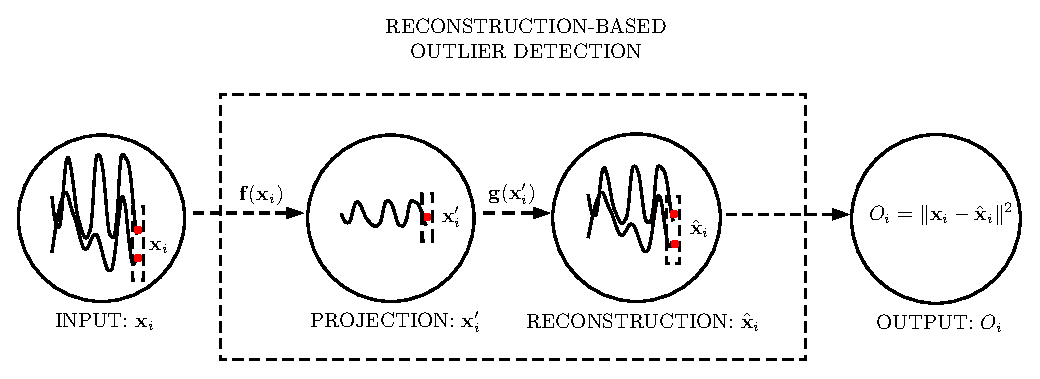
\includegraphics[scale=0.85]{reconstruction-detection/reconstruction_outlierdetection_noexp}
	\caption{General process of reconstruction-based unsupervised online outlier detection in multivariate time series.}
	\label{fig:reconstruction_reconstruction}
\end{figure}

\newpage
\section{Reconstruction-based outlier detection methods}
\label{sec:reconstruction_methods}

A well-known reconstruction-based outlier detection approach, principal component analysis (PCA), learns a linear projection in $k$ orthogonal directions that together capture a large fraction of the variance in the data. Alternative artificial neural networks (ANN) can be used, which typically result in nonlinear functions $\mathbf{f}$ and $\mathbf{g}$ that explicitly minimize the mean squared error. 

\subsection{Principal component analysis}

The basic assumption of PCA, is that our $d$ features likely exhibit linear correlations among each other \cite{aggarwal2015outlier}. If so, we can represent the original $d$-dimensional feature space using only $k$ uncorrelated variables where $k \ll d$. In general, if $\mathbf{X}$ exhibits substantial correlations among the different time series, the first principal components will already explain most of the variation in the original time series \cite{jolliffe1986principal}. The last components will then explain the directions in which only little variation exists and, therefore, probably align well with the outliers we look for.

Outliers in time series are not necessarily characterized by extreme values in any of the original features. Instead, using principal component analysis we can also find outliers that do not conform with the temporal pattern of the remainder of the data. Logically, the analyst is in charge of making an educated guess of the amount of variance needed to explain. Therefore, the number of components $k$ needed to capture the principal temporal patterns should be estimated properly on forehand such that the outliers in $\mathbf{X}$ are not modelled too.

Starting from this intuition, PCA obtains the $k$ principal projection directions by concentrating on an orthonormal linear subspace that maximizes the variance explained in the data. More specifically, it optimizes the $k$ projection directions such that they align with the $k$ (ordered) largest eigenvalues of the covariance matrix of $\mathbf{X}$. For a detailed overview of possible optimization procedures to obtain the projection with PCA, we refer to the work of Jolliffe \cite{jolliffe1986principal}. 

Figure \ref{fig:reconstruction_geometry_projections} illustrates how projecting three data points \{$\mathbf{x}_i : i = 1,2,3$\} in the first principal direction (right), retains the most variance in a $1$-dimensional subspace compared to projecting simply on the y- or x-axis (respectively left and center). 

\begin{figure}[!h]
	\centering
	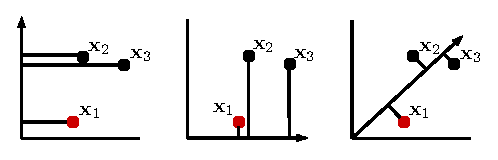
\includegraphics[scale=1.8]{reconstruction-detection/geometry_projections_pca1}
	\caption{Geometric visualization of projections onto the y-axis (left), x-axis (center) and principal direction (right).}
	\label{fig:reconstruction_geometry_projections}
\end{figure}

\newpage
However, in this particular $2$-dimensional case, taking the first principal direction as a model for reconstruction to the original dimensionality might not yield a good base for discriminating outliers. That is, from this projection we expect a good reconstruction of the data point $\mathbf{x}_1$, which could be considered an outlier looking at $\mathbf{x}_2$ and $\mathbf{x}_3$ only. This example reflects the main risk of the PCA-based reconstruction method for outlier detection: if the outliers can be separated well from the principal components used to model the principal behaviour, we can reconstruct our outliers properly resulting in low reconstruction errors and thus low outlier scores. The latter is obviously not what we wish for. 

Clearly, if we extend this example to a feature space with $d \gg 2$, it is crucial to choose the number of projection vectors $k$ carefully in order to make PCA not fit to the outliers. Obtaining a proper $k$-dimensional representation, then, hopefully enables us to separate the outliers by concentrating at data points with the highest reconstruction errors. 

As PCA results in linear projections of the data, $\mathbf{f}$ and $\mathbf{g}$ represent simple matrix multiplications. The projection $\mathbf{x}'$ of $\mathbf{x}$ is obtained from a simple multiplication with all $k$ principal coefficient vectors $\mathbf{w} \in \mathbf{W}$, i.e.

\begin{equation}\label{eq:reconstruction_pcaprojection}
\mathbf{x}' = \mathbf{W} \ \mathbf{x}
\end{equation}

\noindent where $\mathbf{W}$ is called the principal coefficient matrix of size $k \times d$. Then the projected data point $\mathbf{x}'$ can easily be reconstructed to its original dimensionality $d$ using

\begin{equation}\label{eq:reconstruction_pcareconstruction}
\hat{\mathbf{x}} = \mathbf{W}^T \ \mathbf{x}'
\end{equation}  

\noindent taking the transpose $\mathbf{W}^T$ instead of the inverse $\mathbf{W}^{-1}$. We can reconstruct $\mathbf{x}'$ accurately this way, as all $\mathbf{w} \in \mathbf{W}$ are orthogonal to each other and have unit length. That is, we have

\begin{equation}\label{eq:reconstruction_orthonormality}
\mathbf{W}^T \ \mathbf{W} = \mathbf{I}
\end{equation}

\noindent with $\mathbf{I}$ the identity matrix, which is a sufficient condition for accurate reconstruction\footnote{In case the first $k$ components explain the majority of the variance in the data.} using $\mathbf{W}^T$. Outlier scores can be computed as in equation \eqref{eq:reconstruction_score}. A method to conduct approximate principal component analysis online and unsupervised is discussed in section \ref{sec:reconstruction_spirit}. 
 
\vspace{0.2cm}
\subsection{Artificial neural networks}
In some cases, it is infeasible to accurately represent the normal behaviour in a linear lower-dimensional subspace. For those cases, we can resort to nonlinear mappings of the data instead. The objective is to learn a nonlinear function $\mathbf{f} : \mathbb{R}^d \to \mathbb{R}^k$ such that, in turn, the data can be reconstructed by a function $\mathbf{g} : \mathbb{R}^k \to \mathbb{R}^d$. These functions are usually obtained by training an artificial neural network (ANN) on data such that the combination of the two minimize, for example, the mean squared error as in equation \eqref{eq:reconstruction_ann}. 

\begin{equation}\label{eq:reconstruction_ann}
\min_{\mathbf{f},\ \mathbf{g}}\frac{1}{d}\sum\limits_{j=1}^{d}(\mathbf{x}_{j} - \mathbf{g}(\mathbf{f}(\mathbf{x}_{j})))^2
\end{equation}

ANN's are inspired on biological processes taking place in brains to learn representing and reproducing real-world phenomena accurately. Each neuron, or node, in an ANN typically processes its received input (the initial input, or the output of a previous layer) and transmits it to a node in the next layer. Eventually, the ANN is trained to approximate the input by learning its underlying characteristics. Well-known approaches that learn functions $\mathbf{f}$ and $\mathbf{g}$ this way, are autoencoder networks \cite{japkowicz1995novelty} and the multi-layer perceptron \cite{nairac1999system}.

For unsupervised online outlier detection in time series, a recently proposed method combines autoencoders with the principle of variational inference \cite{solch2016variational}. This principle relates to replacing the lower-dimensional encoding $\mathbf{x}'$ of $\mathbf{x}$, and corresponding decoding $\hat{\mathbf{x}}$, with approximations of posterior distributions represented by stochastic variables. The parameters of these stochastic variables are, in turn, learned by recurrent neural networks which capture the temporal dynamics of the time series online.

\newpage
\section{Baseline: online principal component approximation}
\label{sec:reconstruction_spirit}
Though the data at hand might be structured nonlinearly, in this thesis we focus on linear projections of the data. Therefore, we compare the obtained performances to a method approximating the (linear) principal coefficient vectors online, called SPIRIT \cite{papadimitriou2005streaming}. 
Instead of learning the coefficient vectors $\mathbf{w} \in \mathbf{W}$ offline, SPIRIT updates $\mathbf{W}_i$ each time step $i$ to approximate the optimal $k$ orthogonal directions in which the explained variance is maximized. Algorithm \ref{alg:trackw} gives a detailed insight of how the $k$ coefficient vectors are updated over time\footnote{Algorithm \ref{alg:trackw} represents only the update of the projection vectors of the actual algorithm of SPIRIT.}.

In short, the $k$ vectors are updated proportionally to the reconstruction error (step \ref{alg:trackw_op6}) associated with the projection $\mathbf{x}_i'$ onto the $k$ projection vectors at time step $i$ (step \ref{alg:trackw_op4}). The impact of each incoming data point on the updated projection vectors is controlled by a so-called forgetting factor $\lambda$ (steps \ref{alg:trackw_op5} and \ref{alg:trackw_op7}). If $\lambda$ is close to $1$, recent data points have less significant effect on the updates. This way, temporal relations are tracked over time. A suitable range for $\lambda$ to make SPIRIT generalize well to a broad range of applications is [$0.96$, $0.98$] \cite{papadimitriou2005streaming}. 

\begin{algorithm}[H]
	\caption{\quad \textbf{TrackW}}
	\label{alg:trackw}
	\begin{algorithmic}[1]
		\STATE Initialize $k$ coefficient vectors $\mathbf{w}_j$ to unit vectors s.t. $\mathbf{w}_1 = [10\cdots0]$, $\mathbf{w}_2 = [010\cdots0]$, etc. \label{alg:trackw_op1}
		\STATE Initialize $\tilde{\mathbf{x}}_j$ as $\mathbf{x}_i$ \label{alg:trackw_op2}
		\STATE Initialize $d_1$ to a small value between $0$ and $1$
		\label{alg:trackw_op3}
		\FOR{$1 \leq j \leq k$}
		\STATE Project $\tilde{\mathbf{x}}_j$ on $\mathbf{w}_j$ by $x_j' = \mathbf{w}_j \ \tilde{\mathbf{x}}_j$
		\label{alg:trackw_op4}
		\STATE Update $d_j \gets \lambda d_j + (x_j')^2$ \qquad\quad \ \COMMENT{Energy $\propto$ $j$th eigenvalue of $\mathbf{X}_i^T\mathbf{X}_i$}
		\label{alg:trackw_op5}
		\STATE Set $\mathbf{e}_j = \tilde{\mathbf{x}}_j - x_j' \mathbf{w}_j^T $ 
		\label{alg:trackw_op6}
		\STATE Update $\mathbf{w}_j \gets \mathbf{w}_j + \frac{1}{d_j} \ x_j' \ \mathbf{e}_j$ \qquad \COMMENT{Update principal coefficients estimate}
		\label{alg:trackw_op7}
		\STATE $\tilde{\mathbf{x}}_{j+1} \gets \tilde{\mathbf{x}}_j - x_j' \ \mathbf{w}_j^T$
		\label{alg:trackw_op8}
		\ENDFOR
	\end{algorithmic}
\end{algorithm}

Figure \ref{fig:reconstruction_updatew} illustrates the procedure of updating the principal projection directions as soon as a new data point arrives.

\begin{figure}[h]
	\centering
	\vspace{-0.12cm}
	\includegraphics[scale=1]{reconstruction-detection/SPIRIT_updateW}
	\caption{Update procedure of the first estimated principal coefficient vector $\mathbf{w}_1$ for new data point $\mathbf{x}_i$ (in red).}
	\label{fig:reconstruction_updatew}
\end{figure}

Algorithm \ref{alg:spirit} describes the full procedure of how SPIRIT detects outliers in multivariate time series.
Aside from the projection directions, the number of vectors needed to explain the amount of variance as requested by the analyst is updated over time as well\footnote{Technically, the explained variance is estimated. Therefore, this estimated variance is referred to as the `retained energy' of the $k$ coefficient vectors $\mathbf{w} \in \mathbf{W}_i$ denoted by $E_{tot}$.}. SPIRIT takes the bounds reflecting the desired variance to retain as input, which are referred to as $f_{\hat{E}}$ being the lower variance bound and $F_{\hat{E}}$ as the upper variance bound. The variance explained with the $k$ projection vectors at time step $i$ are estimated (step \ref{alg:spirit_op7}), and compared with the provided variance bounds. If the estimated explained variance is lower than these bounds, an additional projection vector is added (\ref{alg:spirit_op8} to \ref{alg:spirit_op10}). If the estimated explained variance is higher than these bounds, the last vector is removed (steps \ref{alg:spirit_op11} to \ref{alg:spirit_op13}).

\vspace{-0.2cm}
\begin{algorithm}[H]
	\vspace{-0.02cm}
	\caption{\quad \textbf{SPIRIT}}
	\label{alg:spirit}
	\vspace{-0.03cm}
	\begin{algorithmic}[1]
		\vspace{-0.025cm}
		\STATE Initialize $k \gets 1$, $E \gets 0$ and $\hat{\mathbf{E}}_1 \gets 0$
		\FOR{${\mathbf x}_i \in {\mathbf X}$}
		\STATE Project $\mathbf{x}_i$ on $\mathbf{W}_i$ by $\mathbf{x}_i' = \mathbf{W}_i \ \mathbf{x}_i$
		\STATE	Set $O_i = \|\mathbf{x}_i - \mathbf{W}_i^T \ \mathbf{x}_i'\|^2$
		\label{alg:spirit_op4}	
		\STATE Update $\mathbf{w}_j \in \mathbf{W}_i$ for $1 \leq j \leq k$ by starting at step \ref{alg:trackw_op2} of algorithm \ref{alg:trackw} 
		\label{alg:spirit_op3}
		\STATE Set $E \gets \frac{(i - 1)E + \|\mathbf{x}_i\|^2}{i}$
		\label{alg:spirit_op5}
		\STATE Update $\hat{\mathbf{E}}_j \gets \frac{(i - 1)\hat{\mathbf{E}}_j + (\mathbf{x}_{i,j}')^2}{i}$ for $1 \leq j \leq k$
		\label{alg:spirit_op6}
		\STATE Estimate retained energy $\hat{E}_{tot} \gets \sum\limits_{j=1}^{k}\hat{\mathbf{E}}_j$
		\label{alg:spirit_op7}
		\IF{$\hat{E}_{tot} < f_{\hat{E}} \ E$}
		\label{alg:spirit_op8}
		\STATE Set $k \gets k + 1$ and $\hat{\mathbf{E}}_{k+1} \gets 0 $
		\label{alg:spirit_op9}
		\STATE add $\mathbf{w}_{k+1}$ to $\mathbf{W}_i$ by starting at step \ref{alg:trackw_op1} of algorithm \ref{alg:trackw}
		\label{alg:spirit_op10}
		\ELSIF{$\hat{E}_{tot} > F_{\hat{E}} \ E$}
		\label{alg:spirit_op11}
		\STATE Set $k \gets k - 1$
		\label{alg:spirit_op12}
		\STATE discard $\mathbf{w}_k$ and $\hat{\mathbf{E}}_k$
		\label{alg:spirit_op13}
		\ENDIF
		\ENDFOR
	\vspace{-0.02cm}	
	\end{algorithmic}
\vspace{-0.1cm}
\end{algorithm}

\vspace{-0.1cm}
The computational complexity of algorithm \ref{alg:spirit} (for each time step $i$) is expressed as $\mathcal{O}(kd)$ \cite{papadimitriou2005streaming}. This means that its runtime mainly depends linearly on the number of components needed to explain the desired fraction of variance between $f_{\hat{E}}$ and $F_{\hat{E}}$, and the number of data points $n$. 
However, though not explicitly included in algorithm \ref{alg:spirit}, the implementation of the algorithm distributed by the authors includes an orthogonalization procedure to obtain an orthonormal $\mathbf{W}_i$ after step \ref{alg:spirit_op3}. Experiments ran without the Gram-Schmidt orthogonalization procedure pointed out we indeed need a strictly orthonormal projection basis $\mathbf{W}_i$ to obtain a good performance for outlier detection purposes. Unfortunately, the need for orthogonalizing $\mathbf{W}_i$ results in a runtime of $\mathcal{O}(k^2d)$ which might be costly if $d$ or $k$ is high. 

Despite the need of orthogonalizing the projection vectors, we selected SPIRIT as a baseline as it is considered tractable for online outlier detection in multivariate time series \cite{aggarwal2015outlier}. Additionally, it runs online without the need for a training phase (supervision). Finally, though not directly a motivation for using SPIRIT as a baseline, taking a linear reconstruction-based method as a baseline makes the intuition behind and understanding of our proposed method easier.

\vspace{-0.1cm}
\section{Open challenges}
\label{sec:reconstruction_challenges}
In this chapter we discussed reconstruction-based outlier detection and identified a few vulnerabilities of such methods, in particular of SPIRIT. Now it is time to make those vulnerabilities more explicit, as they directly led us to the formulation of the objectives of our method.

In figure \ref{fig:reconstruction_geometry_projections}, we illustrated a projection of three data points aligned with the principal direction of those data points. In situations like this one, we would reconstruct our outliers accurately which is the undesired result of using the reconstruction from lower-dimensional representations for outlier detection. 
If we would know the appropriate number of projection vectors to explain the variance of the normal behaviour only, without fitting to the outliers as well, we can count on a good detection performance. However, it is hard to determine variance bounds that generalize well to unseen data streams. Besides, SPIRIT is supposed to run unsupervised, making it impossible to adjust these bounds online. This last resort would also not help for cases where the system behaviour is non-stationary, as one has to adjust these bounds constantly. In general online unsupervised (reconstruction-based) methods for outlier detection are sensitive to parameter settings \cite{aggarwal2015outlier}, introducing the objective to find a method that defeats that challenge for unsupervised online outlier detection. 

Finally, we discussed that SPIRIT in practice might result in a poor computational performance. Going from our problem formulation, we operate in high-dimensional feature spaces for which SPIRIT might not be tractable after all. Especially for outlier detection purposes, we need $\mathbf{W}_i$ to be a strictly orthonormal projection basis, making a costly orthogonalization procedure indispensable. Our second objective regarding the formulated challenges in \ref{tab:intro_characteristics}, therefore, is to improve the runtime performance of $\mathcal{O}(k^2d)$ per time step.


